\subsection{抽象工厂模式(Abstract Factory)}

\subsubsection{抽象工厂模式简介}

抽象工厂模式是一种创建型设计模式,它提供了一种创建相关或依赖对象的最佳方式。在抽象工厂模式中,抽象工厂类声明了创建一组相关或依赖对象的方法,而具体工厂类则实现了抽象工厂类中声明的创建对象的方法。

要实现抽象工厂模式,需要定义一个抽象工厂类来声明创建一组相关或依赖对象的接口,并定义一个具体工厂类来实现抽象工厂类中声明的创建对象的方法。通常,抽象工厂模式中的抽象工厂类和具体工厂类都需要实现一个接口或抽象类,该接口或抽象类定义了一组创建相关或依赖对象的操作。这些操作包括创建对象的方法和一些必要的操作。通过这个接口或抽象类,抽象工厂类和具体工厂类可以定义相同的创建对象的方法,并且可以通过实现该接口或抽象类来实现相同的操作。

抽象工厂模式有一些优点:

抽象工厂模式提供了一种创建一组相关或依赖对象的最佳方式,可以在系统中动态替换产品系列,增强系统的灵活性和可扩展性。
在抽象工厂模式中,客户端不需要关心所创建的具体对象是由哪个具体工厂创建的,只需要知道它所对应的抽象工厂即可。
抽象工厂模式提供了一种更好的扩展方式。

抽象工厂模式也有一些缺点:

在抽象工厂模式中,如果需要增加新的产品,则需要修改抽象工厂类和具体工厂类,这违背了开闭原则。
在抽象工厂模式中,增加新的产品时需要对抽象工厂类进行修改,这会导致抽象工厂类变得臃肿,不利于维护。

通常,抽象工厂模式适用于以下场景:

需要创建一组相关或依赖的对象,且对象的类型由应用程序决定。

需要将对象的创建和对象的使用分离,并且希望在系统中动态替换产品系列。

需要提供一个产品族的产品的接口,而又不指定实际的产品。

抽象工厂模式提供了一种创建一组相关或依赖对象的最佳方式,可以在系统中动态替换产品系列,增强系统的灵活性和可扩展性。因此,如果需要创建一组相关或依赖的对象,并且希望在系统中动态替换产品系列,可以考虑使用抽象工厂模式来实现这个功能。

\subsubsection{抽象工厂模式在项目中的应用}

\begin{figure}[H]
  \centering
  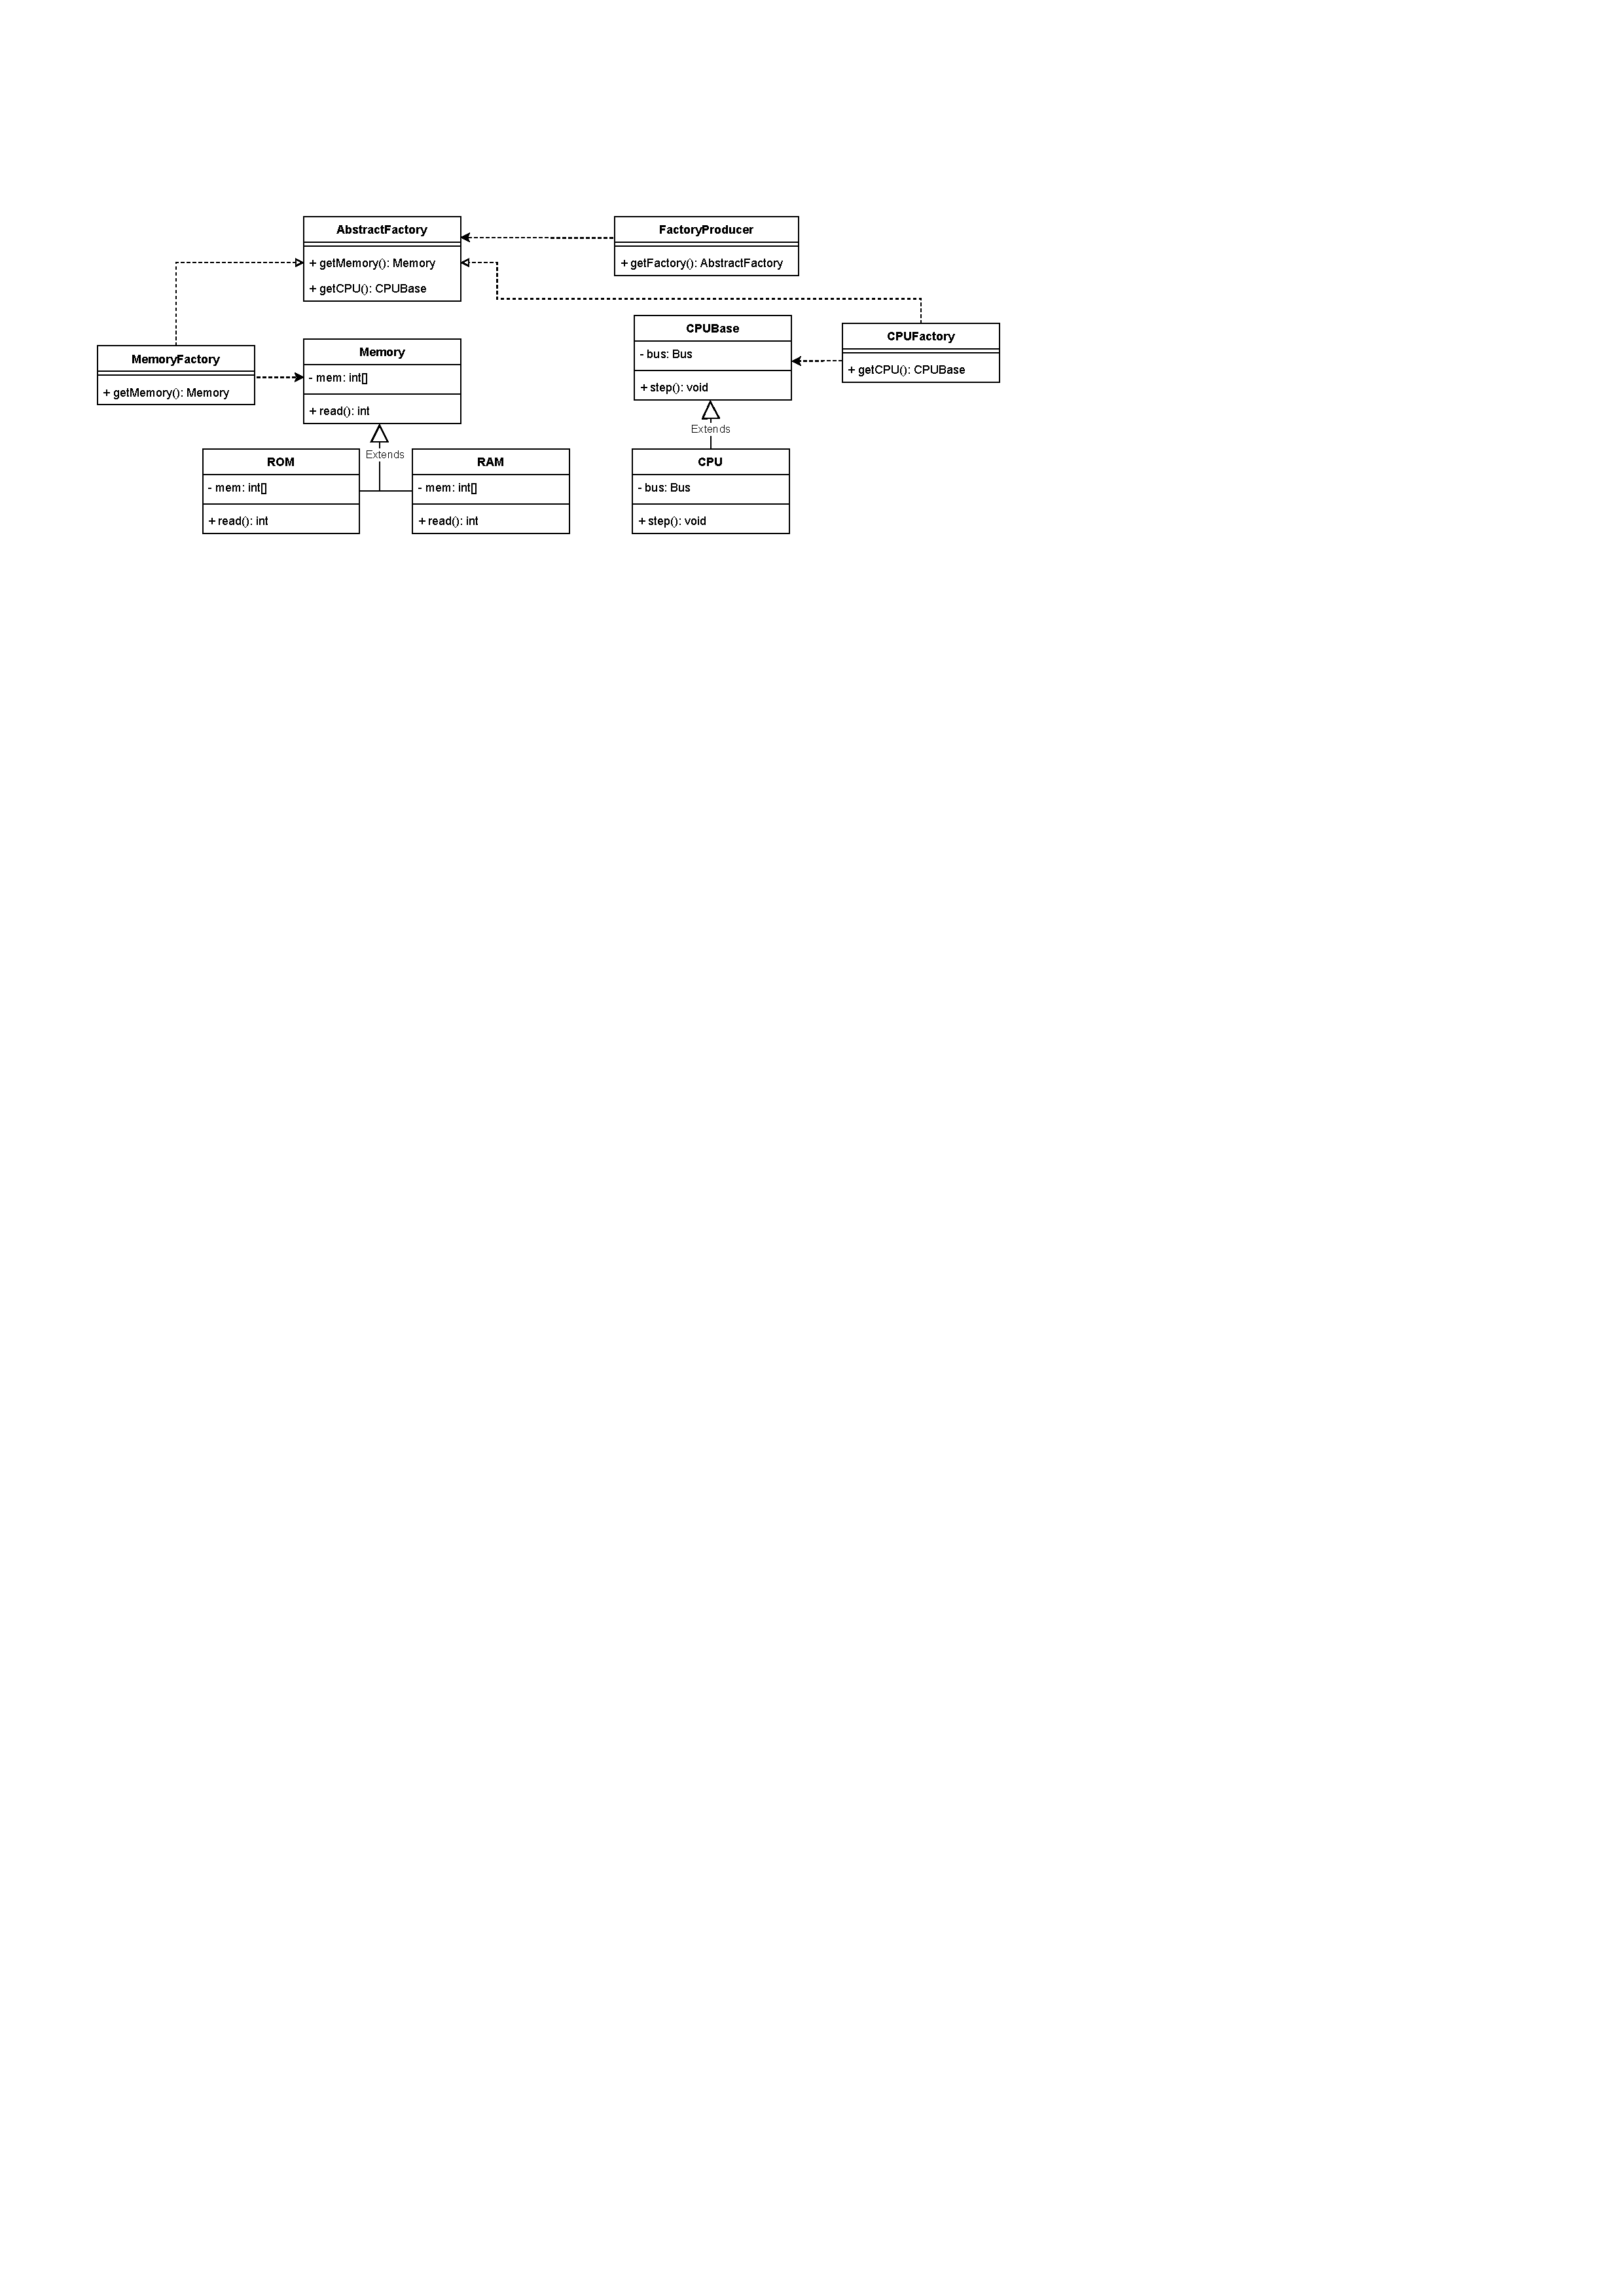
\includegraphics[width=0.9\textwidth]{figures/抽象工厂.pdf}
  \caption{抽象工厂模式在 Slow6502 中的类图}
\end{figure}
